\chapter{Algunos ejemplos y usos}
\graphicspath{{figs/}}

\chapterquote{Que mira bobo}{Lionel Messi, 2023}

\label{C:algunos-ejemplos-y-usos}


%%%%%%%%%%%%%%%%%%%%%%%%%%%%%%%%%%%%%%%%%%%%%%%%%%%%%%%%%%%%%%%%%%%%%%%%
\section{Uso de listas}
\label{S:uso-de-listas}

El problema de la medida se puede describir informalmente del siguiente modo \cite{Bohr1913PMp10}

\begin{enumerate}
    \item hola 1.
        \begin{itemize}
          \item Item 1
          \item Item 2
        \end{itemize}
    \item hola 2.
        \begin{description}
            \item[Item 1:] Descripcion Item 1
            \item[Item 2:] Descripcion Item 2
        \end{description}
    \item hola 3 (ver notas a continuaci\'{o}n) \cite{Bohm1952PRp166,Bohm1952PRp180}:
        \begin{enumerate}
        \item hola a.
        \item hola b.
        \item hola c.
        \end{enumerate}
        
\end{enumerate}


\section{Uso de Imagenes}
\label{S:uso-de-imagenes}
Como incluir una imagen:\\
\begin{figure}[!ht]
\centering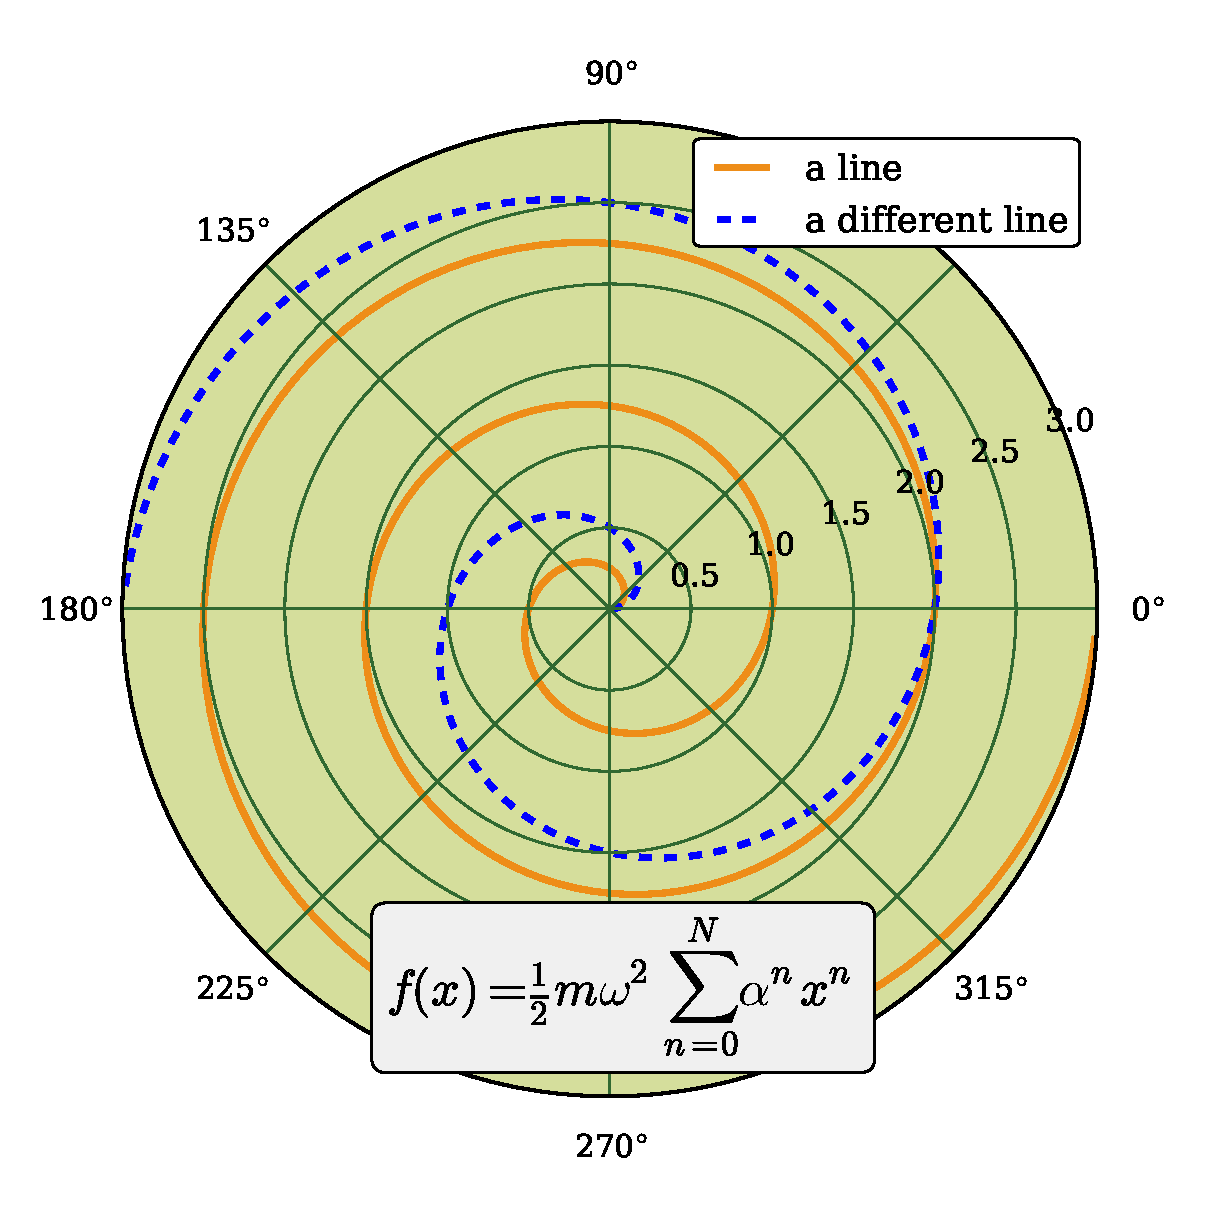
\includegraphics[width=\imsize]{cap2_f1}
\caption[La figura muestra algunas curvas m\'{a}s o menos lindas]{La figura muestra algunas curvas m\'{a}s o menos lindas. El gr\'{a}fico est\'{a} en coordenadas porlares como se muestra en la ref.~\protect{\cite{Hunter07CSE}}}
\end{figure}

\section{Uso de Ecucaciones}
\label{S:uso-de-ecuaciones}
En la primera ecuaci\'{o}n
\begin{equation}
\phi_{1}(z)=A_{1}e^{ik_{1}z}+B_{1}e^{-ik_{1}z}.
\end{equation}

En la segunda ecuaci\'{o}n:
\begin{equation}
\phi_{2}(z)=A_{2}e^{ik_{2}z}+B_{2}e^{-ik_{2}z}.
\end{equation}

\section{Uso de código}
\label{S:uso-de-codigo}

Podemos agregar lineas de código\footnote{\url{https://www.overleaf.com/learn/latex/Code_Highlighting_with_minted}}:
\begin{center}
    \begin{minted}{python}
        for n in range(10):
        if n%2:
        print n
    \end{minted}
\end{center}

También podemos importar código:
\inputminted{python}{cods/holamundo.py}

\section{Uso de circuitikz}
\label{S:uso-de-circuitikz}
Para dibujar circuitos podemos usar Ciruitikz\footnote{\url{https://www.overleaf.com/learn/latex/CircuiTikz_package}}

\begin{figure}[!ht]
    \centering
    \shorthandoff{<>}
    	\begin{circuitikz}[european voltages] \draw
    		(0,0) to [short, *-] (6,0)
                to [V, l_=$\mathrm{j}{\omega}_m \underline{\psi}^s_R$] (6,2) 
                to [R, l_=$R_R$] (6,4) 
                to [short, i_=$\underline{i}^s_R$] (5,4) 
                (0,0) to [open, v^>=$\underline{u}^s_s$] (0,4) 
                to [short, *- ,i=$\underline{i}^s_s$] (1,4) 
                to [R, l=$R_s$] (3,4)
                to [L, l=$L_{\sigma}$] (5,4) 
                to [short, i_=$\underline{i}^s_M$] (5,3) 
                to [L, l_=$L_M$] (5,0);
    	\end{circuitikz}
    \shorthandon{<>}
    \caption{Hola este es el caption del circuito\label{f:ModeloCircuito}}
\end{figure}

%%% Local Variables: 
%%% mode: latex
%%% TeX-master: "main"
%%% End: 
